\documentclass[tikz]{standalone}
\usepackage{amsmath}
\usetikzlibrary{calc}
\definecolor{accent}{HTML}{F7B538}
\definecolor{bg}{HTML}{171D2B}
\begin{document}
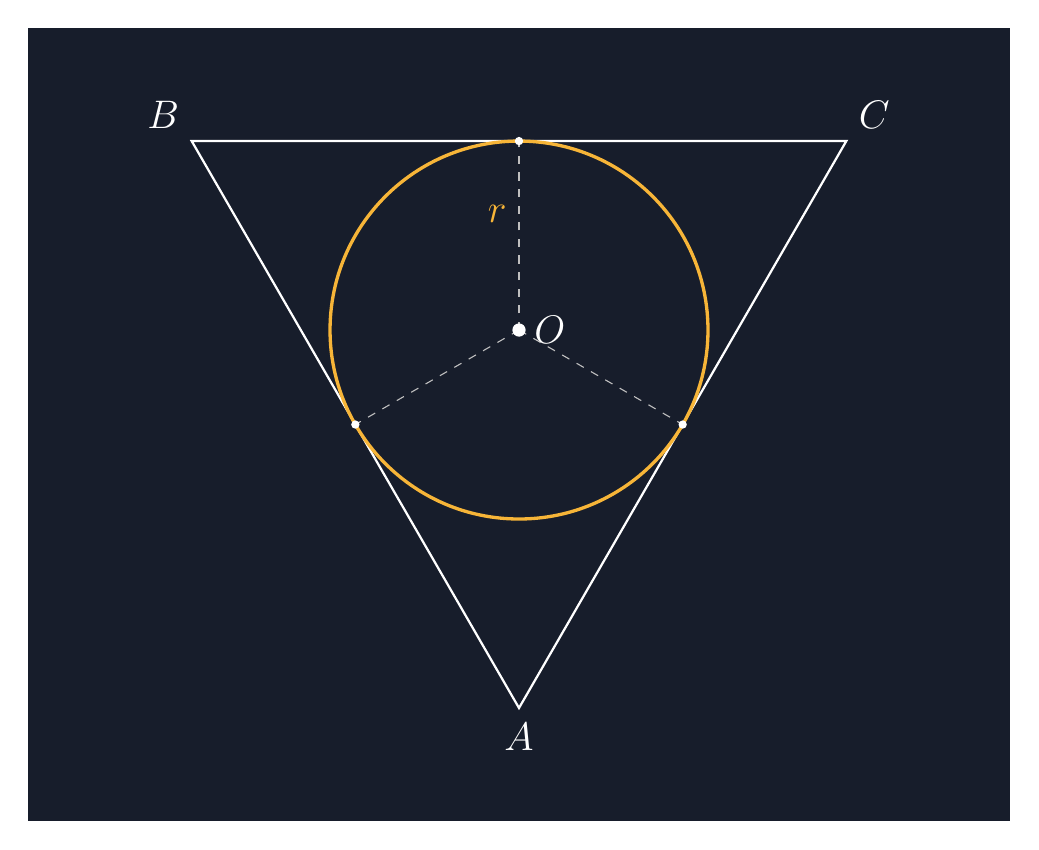
\begin{tikzpicture}[scale=2.4, every node/.style={color=white, font=\Large}]
  \fill[bg] (-2.6,-2.6) rectangle (2.6,1.6);
  \def\R{1}
  \coordinate (O) at (0,0);
  \coordinate (Ta) at (0,1);
  \coordinate (Tb) at (-0.8660,-0.5);
  \coordinate (Tc) at (0.8660,-0.5);
  \coordinate (A) at (0,-2);
  \coordinate (B) at (-1.7320,1);
  \coordinate (C) at (1.7320,1);
  \draw[thick, white] (A) -- (B) -- (C) -- cycle;
  \draw[very thick, accent] (O) circle (\R);
  \draw[dashed, white!75!black] (O) -- (Ta);
  \draw[dashed, white!75!black] (O) -- (Tb);
  \draw[dashed, white!75!black] (O) -- (Tc);
  \fill[white] (O) circle (0.035);
  \node[right=2pt] at (O) {$O$};
  \node[accent, above left=1pt] at ($(O)!0.5!(Ta)$) {$r$};
  \node[above left=1pt] at (B) {$B$};
  \node[above right=1pt] at (C) {$C$};
  \node[below=2pt] at (A) {$A$};
  \fill[white] (Ta) circle (0.022);
  \fill[white] (Tb) circle (0.022);
  \fill[white] (Tc) circle (0.022);
\end{tikzpicture}
\end{document}
